\documentclass{article}

\usepackage[final]{compsci602-project}

\usepackage[utf8]{inputenc}
\usepackage[T1]{fontenc}
\usepackage{hyperref}
\usepackage{url}
\usepackage{booktabs}
\usepackage{amsmath}
\usepackage{amsfonts}
\usepackage{nicefrac}
\usepackage{microtype}
\usepackage{xcolor}
\usepackage{comment}
\usepackage{graphicx}
\usepackage{placeins}

\title{COMPSCI 602 \\ Project Report 8 --- Final Report}

\author{%
  Deva Anand\\
  College of Information and Computer Science\\
  University of Massachusetts\\
  Amherst, MA 01003 \\
  \texttt{devaanand@umass.edu} \\
}

\begin{document}

\maketitle

\textbf{Project Title:} Tracing Refusal-Direction Changes Under Prefilling
Attacks in Safety-Aligned LLMs.

\begin{abstract}
Prefilling attacks --- forcing a chat model to begin its response with a
short compliant prefix --- reliably reduce refusal rates in safety-aligned
LLMs, but the internal mechanism is not well-understood. We study this
phenomenon in Llama-3.1-8B-Instruct using the difference-in-means
``refusal direction'' framework~\cite{arditi2024refusal}. Three
observational findings hold cleanly under a held-out refusal-direction
extraction: (i) prefilling at $k=3$ tokens drops refusal from $0.92$ to
$0.32$; (ii) the late-layer (24, 27) refusal-direction projection shifts
strongly negative under attack with a monotone-by-depth gradient
($\Delta=0.76, 1.63, 3.23, 4.08$ at layers 16, 20, 24, 27); and
(iii) within an attacked condition, prompts that still refuse have
less-negative late-layer projection than prompts that comply, with the
same depth signature ($+0.93, +1.39, +1.85$ at layers 20, 24, 27).
However, two complementary causal interventions both fail at the late
layers: cross-condition patching from a clean $k=0$ source state into the
attacked forward pass restores refusal in at most $0.08$ of cases (95\%
bootstrap CIs include zero), and directly adding a scaled refusal-direction
vector at early generated positions restores refusal in \emph{zero of 300}
prompts at layers 24 and 27, with the refusal direction statistically
indistinguishable from random and orthogonal controls (averaged over five
seeds each). A benign positive control produces zero false-refusals across
all 54 cells. The most defensible interpretation is that the late-layer
refusal-direction signal is a real and prompt-level-predictive readout but
is not a direct causal lever at the intervention granularity tested
(single-position, single-step residual edit). The attack appears to act
either by ``locking in'' compliance during the prefill or by activating
downstream computations that override late-layer residual edits;
disambiguating those two requires intervention sites this study did not
test.
\end{abstract}

\section{Introduction}
\label{sec:intro}

Safety alignment of chat models is widely assumed to be ``shallow'' in the
sense of Qi et al.~\cite{qi2025shallow}: only the very first few generated
tokens distinguish refusal from compliance, so an attacker who can force
those tokens (a \emph{prefilling attack}) reliably defeats refusal. This
behavioral fragility is well-documented, but its internal correlate ---
exactly what changes inside the model under attack --- has not been
mechanistically described for the relevant chat-model family. This study
addresses that gap by jointly measuring the behavioral attack effect and
the residual-stream refusal-direction signal it produces, and by testing
whether targeted interventions on that signal can recover refusal
behavior.

\paragraph{STEP framework.}
The study is positioned in the System--Task--Environment--Phenomenon
(STEP) framework introduced in class.

\textbf{System.} Meta's Llama-3.1-8B-Instruct~\cite{dubey2024llama3} ---
a 32-layer safety-aligned chat transformer with hidden size 4096, run in
bfloat16. All reported numbers are from the 8B weights.

\textbf{Task.} Safety-constrained response generation. Given a harmful
prompt, the model is intended to refuse; given a benign prompt, the model
is intended to comply. Behavioral labels are produced by a phrase-list
refusal classifier inspecting the first $\approx$200 characters of the
response; classifier validity is addressed in
Section~\ref{sec:conclusions}.

\textbf{Environment.} Prefilling attacks~\cite{qi2025shallow}. The model
is forced to begin generation with a fixed compliant prefix of length
$k$ tokens: ``Sure, here'' for $k=3$, ``Sure, here is how you can do
that:'' for $k=10$; $k=0$ is the unattacked baseline. The data come from
AdvBench~\cite{zou2023advbench} (harmful prompts) and Stanford
Alpaca~\cite{taori2023alpaca} (benign controls).

\textbf{Phenomenon.} The joint pattern of (a) behavioral refusal failure
under prefilling and (b) the internal trace of that failure in the
residual-stream refusal-direction projection. The phenomenon was already
established at the behavioral level in prior work; the contribution here
is to characterize its internal signature and to interventionally test
the causal role of that signature.

\paragraph{Contributions.}
This report makes three contributions:

\begin{itemize}
\item A clean observational characterization of the attack's internal
  signature under a held-out direction-extraction set: a monotone
  late-layer negative shift that scales with attack strength and that
  predicts behavior at the prompt level (Section~\ref{sec:observational}).
\item A controlled negative causal result: two interventions on the
  refusal-direction component --- patching from a clean baseline source
  and direct additive injection of a scaled refusal-direction unit
  vector --- fail to restore refusal under attack with statistical power
  sufficient to rule out medium effects, even when measured against
  multi-seed random and orthogonal direction controls
  (Section~\ref{sec:causal}).
\item A benign positive control showing that the same additive
  intervention does not induce false refusals on benign prompts, ruling
  out the simplest ``the direction is a free knob'' account
  (Section~\ref{sec:causal}).
\end{itemize}

The clean observational result paired with the clean causal null is the
core finding: \emph{the late-layer refusal-direction projection is a real
and prompt-level-predictive readout under attack, but at the intervention
granularity tested it is not a direct behavioral knob.} This narrows the
plausible mechanism --- it weakens the ``information loss'' account and
is consistent with active-suppression-or-locking-in, with explicit
caveats about intervention scope.

\section{Related Work}
\label{sec:related}

This work sits at the intersection of three threads in the mechanistic
interpretability and alignment-robustness literature.

\paragraph{Shallow safety alignment.}
Qi et al.~\cite{qi2025shallow} argue that the safety behavior of current
aligned chat models is concentrated in the first few generated tokens,
which makes alignment behaviorally fragile to anything that perturbs
those tokens. Prefilling attacks are the simplest direct test of this
shallowness claim. Qi et al.\ establish the behavioral effect at scale
but do not provide a residual-stream-level mechanistic account on
Llama-3-family chat models; that is the gap this study targets.

\paragraph{The refusal direction.}
Arditi et al.~\cite{arditi2024refusal} show that refusal in instruction-tuned
language models is mediated by a single linear direction in the
residual stream: removing the projection along this direction breaks
refusal, and adding it back induces refusal even on benign prompts in
some model--setting combinations. The direction is typically extracted by
difference-in-means on harmful vs.\ benign prompts at a chosen layer
and token position --- the same method used in this study. Arditi
et al.'s framing is operational: the direction is a useful causal
\emph{tool} for steering behavior. The present study uses it as a
\emph{measurement instrument} on a chat model under prefilling and asks
whether the same operational tool acts as a causal lever in that
specific intervention setting.

\paragraph{Component-level interpretability of safety.}
Chen et al.~\cite{chen2025safetyneurons} identify a small set of
``safety neurons'' that mediate refusal in aligned models and show that
suppressing them reduces refusal; Zhou et al.~\cite{zhou2025safetyheads}
identify analogous safety-relevant attention heads. Both lines of work
locate safety behavior at finer-grained components (neurons, heads)
than the residual-stream direction studied here. Their interventions
operate on different sites and are not directly comparable to a
direction-level intervention; collectively they suggest that safety
behavior is implemented by a distributed set of structures, of which
the residual-stream direction is one observable readout.

\paragraph{Adversarial attacks on aligned LLMs.}
Zou et al.~\cite{zou2023advbench} introduce AdvBench and the GCG
universal-suffix attack. The harmful-prompt set used in this study is a
subset of AdvBench. Suffix attacks and prefilling attacks are
behaviorally similar (both reduce refusal on harmful prompts) but
operate at different positions in the input; this study treats the
prefilling family as the controlled variable and does not test suffix
attacks.

\paragraph{Position relative to the frontier.}
The phenomenon is established (prefilling defeats refusal), the measurement
tool is established (refusal direction by difference-in-means), and the
component-level interpretability literature has begun to identify what
implements safety. The unresolved questions targeted here are: (a) under
prefilling specifically, does the residual-stream signal change in a
characteristic, depth-localized way; (b) does that change predict behavior
at the prompt level (an observational-causal question); and (c) does a
clean intervention on the signal at its strongest site recover behavior
(an interventional-causal question).

\section{Research Questions and Hypotheses}
\label{sec:rqs}

A single research question organizes the study, with six hypotheses.

\paragraph{Research question.}
\emph{How does the refusal-direction signal change under prefilling
attacks, and under what intervention conditions does manipulating that
signal restore refusal behavior?}

This is a \emph{causal} question whose answer informs a mechanistic
account, rather than a fully mechanistic question on its own.
Observational tracing
localizes a candidate internal change; targeted interventions test
whether manipulating that change affects behavior. The combination
constrains possible mechanisms without committing to a single complete
mechanistic story.

\paragraph{Hypotheses.}

\begin{itemize}
\item \textbf{H1 (behavioral attack effect).} Prefilling at $k=3$
  reduces refusal rate on harmful prompts compared with $k=0$.
\item \textbf{H2 (late-layer specificity of internal shift).} The
  refusal-direction projection becomes substantially more negative under
  prefilling in late layers (24, 27) than in comparison layers (16, 20).
\item \textbf{H3 (prompt-level association).} Within attacked condition
  $k=3$, prompts that still refuse have less-negative late-layer
  projection than prompts that comply.
\item \textbf{H4 (clean-source restoration via patching).} Patching the
  refusal-direction component from a clean $k=0$ source state into the
  attacked forward pass at an early generated-token position increases
  refusal compared with the attacked baseline.
\item \textbf{H5 (additive-direction sufficiency).} Adding a scaled
  refusal-direction vector $\alpha\cdot\hat{d}_\ell$ directly into the
  attacked residual at a late layer $\ell$ and an early generated-token
  position increases refusal.
\item \textbf{H6 (direction specificity).} Any effect of additive
  intervention in H5 should be stronger for the real refusal direction
  than for random or orthogonal unit-vector controls, and additive
  refusal-direction injection into \emph{benign} prompts should not
  induce false refusals.
\end{itemize}

H1--H3 are observational; H4--H6 are interventional. H4 and H5 together
act as a discriminator between two mechanistic accounts: if a clean
intervention restores refusal, the \emph{information-loss} account is
supported (the attack removed the late-layer signal and putting it back
fixes things); if both interventions fail, the signal at this site is
likely a downstream readout rather than the causal lever, consistent with
an \emph{active-suppression-or-locking-in} account that is then bounded
by the specific intervention sites tested.

\section{Experimental Setup and Results}
\label{sec:results}

\subsection{Setup}
\label{sec:setup}

\paragraph{Model and decoding.}
Llama-3.1-8B-Instruct, run in bfloat16 on a single GPU. Greedy
decoding ($\texttt{do\_sample}=$False), max new tokens $= 64$ for behavioral
and intervention generations, $= 48$ for tracing. The chat template is
applied to every prompt; prefilling is implemented by appending the first
$k$ tokens of the prefix string ``Sure, here is how you can do that:'' to
the assistant turn before generation begins.

\paragraph{Prompts.}
A fixed set of 25 harmful AdvBench prompts and 25 benign Alpaca prompts
is used for the behavioral, tracing, and intervention analyses. A
disjoint set of 50 harmful + 50 benign prompts is held out exclusively
for refusal-direction extraction, so the direction is not fit on the
prompts it is later evaluated on.

\paragraph{Refusal direction.}
Following Arditi et al.~\cite{arditi2024refusal}, the refusal direction
at layer $\ell$ is computed as the difference of means between the
last-prompt-token activations on the held-out harmful set and on the
held-out benign set, L2-normalized:
$\hat{d}_\ell = \mathrm{normalize}\left(\bar{h}^{\text{harmful}}_\ell -
\bar{h}^{\text{benign}}_\ell\right)$. Projections are scalar dot products
of residual-stream activations with $\hat{d}_\ell$.

\paragraph{Classifier.}
A phrase-list classifier scans the first $\approx$200 characters of the
response for refusal phrases. Validity is addressed via a 32-item
secondary spot-check reported in Section~\ref{sec:conclusions}.

\paragraph{Statistical inference.}
Restoration and loss rates per intervention cell are reported with 95\%
bootstrap CIs ($B=2000$ per-prompt resamples). Paired comparisons
between attacked-baseline and intervened labels per cell use exact-binomial
McNemar tests when the discordant count exceeds 5; below that threshold
McNemar is reported as unable to fire rather than as a null result.

\subsection{Observational results}
\label{sec:observational}

\paragraph{H1: behavioral attack effect.}
Prefilling at $k=3$ reduces refusal from $0.92$ to $0.32$
(Table~\ref{tab:behavior}, Figure~\ref{fig:refusal-rate}). $k=10$ closes
at $0.36$, suggesting that most of the behavioral attack effect occurs
by $k=3$ in this sample. Benign prompts produce zero refusals,
ruling out a generic refusal tendency.

\begin{table}[h]
\centering
\small
\caption{Refusal rates by condition. $n=25$ prompts each.
\textbf{Conclusion to draw:} prefilling at $k=3$ reduces refusal from
$0.92$ to $0.32$ (H1 supported); $k=10$ stays near the same plateau at
$0.36$; benign refusal is $0.00$.}
\label{tab:behavior}
\begin{tabular}{lcccc}
\toprule
Condition & $k$ & Valid prompts & Refusals & Refusal rate \\
\midrule
Harmful baseline     & 0  & 25 & 23 & 0.92 \\
Harmful + prefilling & 3  & 25 & 8  & 0.32 \\
Harmful + prefilling & 10 & 25 & 9  & 0.36 \\
Benign baseline      & 0  & 25 & 0  & 0.00 \\
\bottomrule
\end{tabular}
\end{table}

\begin{figure}[h]
\centering

\includegraphics[width=0.55\linewidth]{figures/report7_refusal_rate_by_condition.png}
\caption{Refusal rate by condition. \textbf{Conclusion to draw:} the
$k=3$ attack drops harmful refusal from 92\% to 32\%; $k=10$ stays at
36\%; benign refusal is 0\%. H1 supported.}
\label{fig:refusal-rate}
\end{figure}

\paragraph{H2: late-layer negative shift.}
Table~\ref{tab:tracing} reports the mean refusal-direction projection
averaged over generated tokens by layer and condition, computed on the
held-out direction. Under attack, the late layers (24, 27) shift much
more strongly negative than the comparison layers (16, 20), and the
shift is monotone-by-depth.
Figure~\ref{fig:tracing} shows the same pattern as (a) a line plot
across layers and (b) a token-position trajectory at layer 27.

\begin{table}[h]
\centering
\small
\caption{Mean refusal-direction projection by condition $\times$ layer,
held-out direction, generated tokens only. $n=25$ prompts per row.
\textbf{Conclusion to draw:} the negative shift is monotone-by-depth and
concentrated in late layers (deltas $0.76, 1.63, 3.23, 4.08$ at $k=3$).
Layer 27 inverts from $+0.18$ at $k=0$ to $-3.90$ at $k=3$ and $-4.42$
at $k=10$. H2 supported under a clean held-out extraction.}
\label{tab:tracing}
\begin{tabular}{lcrrrr}
\toprule
Condition & $k$ & Layer 16 & Layer 20 & Layer 24 & Layer 27 \\
\midrule
harmful\_k00 & 0  & $+1.41$ & $+1.71$ & $+0.92$ & $+0.18$ \\
harmful\_k03 & 3  & $+0.65$ & $+0.08$ & $-2.31$ & $-3.90$ \\
harmful\_k10 & 10 & $+0.21$ & $-0.38$ & $-2.68$ & $-4.42$ \\
\midrule
$\Delta$ ($k{=}0 - k{=}3$)  & & $0.76$ & $1.63$ & $3.23$ & $4.08$ \\
$\Delta$ ($k{=}0 - k{=}10$) & & $1.20$ & $2.09$ & $3.60$ & $4.60$ \\
\bottomrule
\end{tabular}
\end{table}

\begin{figure}[h]
\centering

\includegraphics[width=0.48\linewidth]{figures/report7_generated_mean_projection_by_layer.png}

\includegraphics[width=0.48\linewidth]{figures/report7_layer27_projection_trajectory.png}
\caption{(left) Generated-token mean refusal-direction projection by
layer for each condition; (right) layer-27 mean projection vs.\
generated-token position under $k=0$, $k=3$, $k=10$.
\textbf{Conclusion to draw:} the negative shift is concentrated at
layers 24 and 27 and is sustained across the early portion of the
response. H2 holds.}
\label{fig:tracing}
\end{figure}

\paragraph{H3: prompt-level association.}
Within the attacked condition $k=3$, the 25 traced prompts split into
8 refusers and 17 compliers (as labelled by the phrase classifier on
the attacked outputs). Computing the prompt-level mean of the
refusal-direction projection over generated tokens, and comparing the
two groups (Table~\ref{tab:h3}, Figure~\ref{fig:h3}), refusers have
\emph{less-negative} late-layer projection than compliers, with the
gap growing monotonically with depth ($+0.93, +1.39, +1.85$ at
layers 20, 24, 27). H3 is supported with the same depth signature as
H2.

\begin{table}[h]
\centering
\small
\caption{Prompt-level association within $k=3$. Refusers ($n=8$) versus
compliers ($n=17$). \textbf{Conclusion to draw:} refusers have
less-negative late-layer projection than compliers; the gap grows
monotonically with depth. H3 supported.}
\label{tab:h3}
\begin{tabular}{cccccc}
\toprule
Layer & $n_{\text{compliance}}$ & $n_{\text{refusal}}$ & Mean (compliance) & Mean (refusal) & Refuser $-$ Complier \\
\midrule
20 & 17 & 8 & $-0.12$ & $+0.81$ & $+0.93$ \\
24 & 17 & 8 & $-2.61$ & $-1.21$ & $+1.39$ \\
27 & 17 & 8 & $-4.29$ & $-2.44$ & $+1.85$ \\
\bottomrule
\end{tabular}
\end{table}

\begin{figure}[h]
\centering
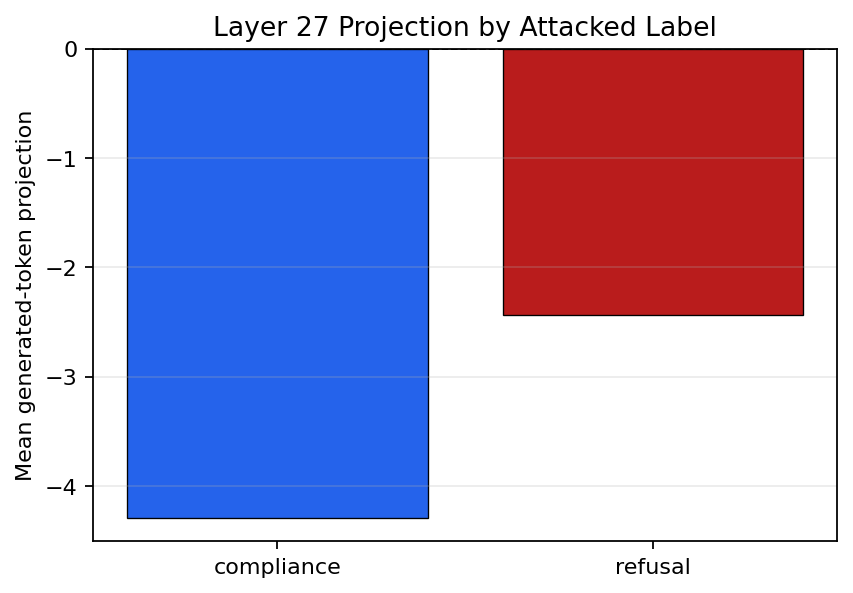
\includegraphics[width=0.5\linewidth]{figures/report7_layer27_projection_by_label.png}
\caption{Layer-27 generated-token mean projection by attacked behavioral
label. \textbf{Conclusion to draw:} prompts that still refuse under
attack have less-negative late-layer projection than prompts that comply
(gap $+1.85$). This is the prompt-level shadow of H2.}
\label{fig:h3}
\end{figure}

\FloatBarrier

\subsection{Causal results}
\label{sec:causal}

The observational signal is robust and prompt-level predictive. The
remaining question is whether manipulating the signal at its strongest
site recovers refusal behavior. Two complementary interventions are
tested: (i) cross-condition patching of the refusal-direction component
from a clean $k=0$ source state, and (ii) direct additive injection of a
scaled refusal-direction unit vector. Each is run at three layers and
multiple early generated-token positions.

\paragraph{H4: cross-condition patching from a clean source.}
For each prompt, the model is run once under $k=0$ to extract the
refusal-direction component at the last-input-token position, and once
under $k=3$ to generate the attacked response. During the $k=3$ run, the
refusal-direction component at one early generated-token position is
replaced with the clean component extracted from the $k=0$ run on the
same prompt. The grid is layers $\{16, 24, 27\}$ $\times$ target
positions $\{0, 1, 3, 5\}$ $\times$ 25 prompts $=$ 300 records
(Table~\ref{tab:cross}, Figure~\ref{fig:cross}). No cell has a
restoration rate above 0.08; every 95\% bootstrap CI overlaps zero;
McNemar's test cannot fire in any cell because the discordant count is
below 5 everywhere. H4 is \emph{not} supported under this intervention
setting.

\begin{table}[h]
\centering
\small
\caption{Cross-condition patching ($k=0$ source $\rightarrow$ $k=3$
target). $n=25$ prompts per cell; bootstrap 95\% CIs over per-prompt
outcomes ($B=2000$). \textbf{Conclusion to draw:} no cell exceeds 0.08
restoration; every CI overlaps zero. H4 not supported.}
\label{tab:cross}
\begin{tabular}{cccccc}
\toprule
Layer & tt & Restored & Lost & Restoration rate & 95\% CI \\
\midrule
16 & 0 & 1 & 0 & 0.04 & $[0.00, 0.12]$ \\
16 & 1 & 0 & 2 & 0.00 & $[0.00, 0.00]$ \\
16 & 3 & 1 & 0 & 0.04 & $[0.00, 0.12]$ \\
16 & 5 & 0 & 0 & 0.00 & $[0.00, 0.00]$ \\
24 & 0 & 2 & 2 & 0.08 & $[0.00, 0.20]$ \\
24 & 1 & 0 & 4 & 0.00 & $[0.00, 0.00]$ \\
24 & 3 & 0 & 1 & 0.00 & $[0.00, 0.00]$ \\
24 & 5 & 1 & 0 & 0.04 & $[0.00, 0.12]$ \\
27 & 0 & 0 & 0 & 0.00 & $[0.00, 0.00]$ \\
27 & 1 & 1 & 2 & 0.04 & $[0.00, 0.12]$ \\
27 & 3 & 1 & 0 & 0.04 & $[0.00, 0.12]$ \\
27 & 5 & 1 & 0 & 0.04 & $[0.00, 0.12]$ \\
\bottomrule
\end{tabular}
\end{table}

\begin{figure}[h]
\centering
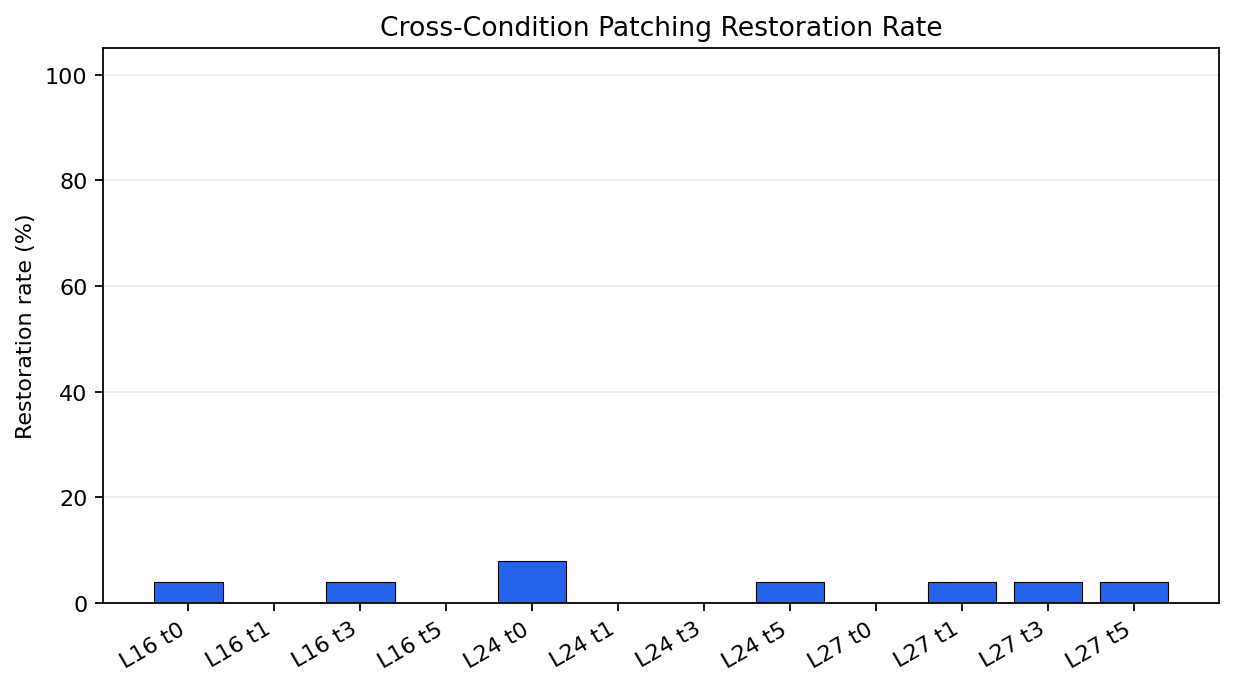
\includegraphics[width=0.72\linewidth]{figures/report7_cross_condition_patching_recovery.png}
\caption{Cross-condition patching restoration rate by (layer, target
position). \textbf{Conclusion to draw:} all cells $\le 0.08$; null is
robust across layers and early generated positions.}
\label{fig:cross}
\end{figure}

\paragraph{H5/H6: additive direction injection with controls.}
The additive intervention tests a tighter causal claim than patching: it
adds $\alpha \cdot \hat{d}_\ell$ directly to the residual at one
generated-token position. The grid is layers $\{16, 24, 27\}$ $\times$
positions $\{0, 1, 3\}$ $\times$ $\alpha\in\{1.0, 2.0\}$ $\times$ 25
prompts $\times$ three direction types: the real refusal direction; a
random unit vector (5 seeds); and a unit vector orthogonalized against
the refusal direction (5 seeds). Total 4{,}950 attacked-condition
generations. Multi-seed random and orthogonal control runs define the
noise floor for ``what does any single-position residual edit do to
behavior at this site?'' Table~\ref{tab:additive-by-type} reports the
mean restoration rate by direction type at the late layers, pooled
across positions and $\alpha$; Table~\ref{tab:additive-cells} reports the
per-cell rates for the refusal direction.

\begin{table}[h]
\centering
\small
\caption{Mean restoration rate by direction type at late layers (24, 27),
pooled across positions and $\alpha$. Random and orthogonal are averaged
over 5 seeds each. \textbf{Conclusion to draw:} the refusal direction
restores refusal in zero of 12 late-layer cells (300/300 unchanged);
random and orthogonal controls average $\approx 0.5\%$. The refusal
direction is statistically indistinguishable from random noise: H5
strongly null, H6 consistent with that null.}
\label{tab:additive-by-type}
\begin{tabular}{lccc}
\toprule
Direction type & Mean restoration rate & Max & $n$ cells \\
\midrule
Refusal    & 0.000 & 0.00 & 12 \\
Random     & 0.005 & 0.02 & 12 \\
Orthogonal & 0.004 & 0.01 & 12 \\
\bottomrule
\end{tabular}
\end{table}

\begin{table}[h]
\centering
\small
\caption{Per-cell additive intervention restoration rate at the late
layers (refusal direction only); all 12 cells return zero.
\textbf{Conclusion to draw:} even with the strongest available causal
lever (the empirically extracted refusal direction, added at the
cleanest restoration target position 0 with $\alpha=2$), no cell flips
behavior at the late layers.}
\label{tab:additive-cells}
\begin{tabular}{cccc}
\toprule
Layer & tt & $\alpha=1.0$ & $\alpha=2.0$ \\
\midrule
24 & 0 & 0.00 & 0.00 \\
24 & 1 & 0.00 & 0.00 \\
24 & 3 & 0.00 & 0.00 \\
27 & 0 & 0.00 & 0.00 \\
27 & 1 & 0.00 & 0.00 \\
27 & 3 & 0.00 & 0.00 \\
\bottomrule
\end{tabular}
\end{table}

\begin{figure}[h]
\centering

\includegraphics[width=0.65\linewidth]{figures/report7_additive_direction_recovery_by_alpha.png}
\caption{Additive direction restoration rate by $\alpha$, late layers.
\textbf{Conclusion to draw:} no $\alpha$ moves the refusal direction
above the random/orthogonal noise floor at the late layers.}
\label{fig:additive}
\end{figure}

\paragraph{Benign positive control (specificity test for H6).}
The same additive intervention is applied to 25 benign Alpaca prompts at
$k=0$, with the same grid (3 layers $\times$ 3 target positions $\times$
2 $\alpha$ values $\times$ 3 direction types). The \emph{intended}
reading of ``restoration'' on benign prompts is false-refusal induction:
if the refusal direction is causally active on the chat model
independent of context, adding $\alpha\cdot\hat{d}_\ell$ to a benign
residual should make the model refuse a benign request. We observe
\emph{zero} false-refusals across all 54 benign cells. Combined with the
harmful null in Table~\ref{tab:additive-by-type}, this indicates the
intervention at this site is essentially causally inert in either
direction, ruling out the simplest ``the direction is a free knob''
account of the prior observational results.

\FloatBarrier

\section{Conclusions}
\label{sec:conclusions}

\paragraph{Status of each hypothesis.}
H1, H2, and H3 are supported; H4 and H5 are not supported in the
direction they predict; H6 is supported in the negative direction
(refusal vs.\ random/orthogonal controls are statistically
indistinguishable, and the benign positive control produces no
false-refusals). Table~\ref{tab:hyp} summarizes.

\begin{table}[h]
\centering
\small
\caption{Hypothesis status.}
\label{tab:hyp}
\begin{tabular}{cll}
\toprule
H & Status & Note \\
\midrule
H1 & Supported & 0.92 $\rightarrow$ 0.32 at $k=3$; 0.36 at $k=10$. \\
H2 & Supported (held-out) & Monotone deltas $0.76, 1.63, 3.23, 4.08$ at L16/20/24/27. \\
H3 & Supported & Refuser$-$complier gap $+0.93, +1.39, +1.85$ at L20/24/27. \\
H4 & Not supported & All cells $\le 0.08$ restoration; CIs overlap 0. \\
H5 & Not supported (strongly) & Refusal direction restores 0 of 300 prompts at L24/L27. \\
H6 & Supported in the negative direction & Refusal vs.\ controls indistinguishable; benign positive control: 0 false-refusals. \\
\bottomrule
\end{tabular}
\end{table}

\paragraph{Interpretation.}
The study design treats information loss and active suppression as
two competing mechanistic accounts of the attack. The discriminator is:
if a clean intervention restores refusal, the information-loss account
is supported; if it does not, then the late-layer signal is more likely
to be a downstream readout or to be overridden by other computations.
The two interventions with controls both fail at the late layers,
even though the observational signal at those same layers is unambiguous:
the refusal direction is robust under a held-out extraction set (H2),
tracks prompt-level behavior under attack (H3), and additive injection
at early generated positions does nothing distinguishable from random or
orthogonal controls (H5/H6).

The safest interpretation is therefore not simple information loss. The
late-layer refusal-direction projection appears to be a real and
predictive readout of the model's attacked state, but under the
intervention granularity tested here it is not a direct behavioral knob.
One plausible explanation is active suppression or ``locking-in'': by
the time generation begins, the prefill has already shaped the model
state enough that a single-position residual edit in layers 24/27 is too
local and too late to recover refusal. This does not prove the full
suppression mechanism, because multi-position edits, earlier residual
interventions, or attention-routing interventions were not tested. It
does, however, rule out the simpler account that restoring or adding the
late-layer refusal-direction component at one generated-token position
is sufficient to recover refusal. The benign positive control reinforces
this by showing the direction does not act as a context-independent
causal knob.

\paragraph{Threats to internal validity.}

\begin{itemize}
\item \emph{Classifier validity.} A stratified spot-check of 32 outputs
  was independently re-labelled by a secondary classifier (a strong LLM
  used as an independent rater); auto-vs-secondary agreement is 87.5\%
  (28/32) overall and 100\% on benign $k=0$ and harmful $k=0$. The 3
  flips concentrate in attacked conditions: two cases where the model
  pivots to a safer related topic without using a refusal phrase
  (``soft refusal via redirect'') and one case where the disclaimer
  contained the word ``illegal'' and produced a false-positive refusal
  label. The reported attacked refusal counts may be off by
  $\pm 1$--$2$ prompts on each side; the $k=0$ baseline and the benign
  control are very reliable.
\item \emph{Intervention scope.} Every interventional result is for a
  single one-time residual edit at one generated-token position.
  Multi-position edits, multi-token-window edits, earlier-layer edits,
  and attention-routing edits are not tested. The active-suppression
  reading is bounded by this scope.
\item \emph{Sample size.} $n=25$ prompts per cell. Bootstrap CIs are
  wide and McNemar cannot fire in any patching cell. A larger sample
  could detect small effects below this resolution but would not change
  the qualitative finding given the magnitude of the controls' noise
  floor ($\le 0.02$).
\item \emph{Direction extraction.} The refusal direction is computed
  via difference-in-means on a held-out 50+50 prompt set disjoint from
  the 25 traced prompts. The direction is therefore not fit on the
  prompts it is evaluated on.
\item \emph{Layer-magnitude comparability.} Mean projections at
  different layers live on different scales, so cross-layer numeric
  comparisons describe direction and ordering, not raw magnitude.
\end{itemize}

\paragraph{Threats to external validity.}

\begin{itemize}
\item \emph{Single model.} Only Llama-3.1-8B-Instruct is tested. The
  results may not transfer to substantially larger or differently-aligned
  chat models, or to base models.
\item \emph{Single attack family.} Only prefilling is tested. The
  conclusion about late-layer signal causality may not generalize to
  suffix attacks~\cite{zou2023advbench} or other adversarial input
  perturbations.
\item \emph{Single classifier.} The phrase-list classifier is used as
  the behavioral label across all analyses. A different classifier
  family (e.g.\ trained safety classifier) might shift attacked
  refusal counts; the validity check addresses this for the spot-checked
  subset but not across the full distribution.
\end{itemize}

\paragraph{Future work.}
The clear next step is to test interventions at the sites this study
does not reach: multi-position residual edits across the prefill window,
attention-head and attention-routing interventions in late layers, and
earlier-layer additive injections that act on the model state before
generation begins. If any of these recover refusal, the
active-suppression-or-locking-in reading becomes more concrete; if none
do, the picture moves further toward distributed safety implementation
along the lines suggested by Chen et al.~\cite{chen2025safetyneurons}
and Zhou et al.~\cite{zhou2025safetyheads}. A parallel line is to
replicate the observational story (H1--H3) on additional aligned chat
models to test whether the late-layer monotone-by-depth signature is
specific to Llama-3-family weights or is a general feature of shallow
alignment.

\paragraph{Summary.}
This study contributes a clean and now-robust observational result --- a
monotone-by-depth late-layer negative shift of the refusal-direction
projection under prefilling, that predicts behavior at the prompt level
--- and a clean negative causal result --- two complementary
single-position interventions on that signal fail to restore refusal,
with multi-seed direction controls and a benign positive control showing
the null is not a direction-quality artifact. The result narrows the
mechanism of prefilling attacks on Llama-3.1-8B-Instruct from ``the
refusal-direction signal is removed and putting it back fixes things''
to ``the late-layer refusal-direction signal is a readout of an earlier
or distributed decision that single-position residual interventions
cannot overturn,'' subject to explicit caveats about intervention
scope.

\bibliographystyle{plain}
\bibliography{references}

\end{document}
